\documentclass[12pt]{article}
\usepackage[utf8]{inputenc} 
% \usepackage[french]{babel}
\usepackage{graphicx} \graphicspath{{./img/}}
\usepackage{amsmath,amssymb,amsthm} 
% \usepackage{algorithm,algorithmic}
\usepackage{caption}
\usepackage{subcaption}

\usepackage[left=3cm,right=3cm,top=2cm,bottom=2cm]{geometry}
\usepackage{url} 
\usepackage[T1]{fontenc} 
\usepackage{xcolor}
\usepackage{float}
\usepackage{listings}
\lstset{ %
language=C++,                % choose the language of the code
basicstyle=\footnotesize,       % the size of the fonts that are used for the code
numbers=left,                   % where to put the line-numbers
numberstyle=\footnotesize,      % the size of the fonts that are used for the line-numbers
stepnumber=1,                   % the step between two line-numbers. If it is 1 each line will be numbered
numbersep=5pt,                  % how far the line-numbers are from the code
backgroundcolor=\color{white},  % choose the background color. You must add \usepackage{color}
showspaces=false,               % show spaces adding particular underscores
showstringspaces=false,         % underline spaces within strings
showtabs=false,                 % show tabs within strings adding particular underscores
frame=single,           % adds a frame around the code
tabsize=2,          % sets default tabsize to 2 spaces
captionpos=b,           % sets the caption-position to bottom
breaklines=true,        % sets automatic line breaking
breakatwhitespace=false,    % sets if automatic breaks should only happen at whitespace
escapeinside={\%*}{*)}          % if you want to add a comment within your code
}

\usepackage{hyperref}
\hypersetup{colorlinks=true}

\newcommand\hsp{\hspace{1.0cm}}

\begin{document}
\begin{titlepage}
\begin{center}
\vspace*{3cm}
\textsc{\Large Rapport}\\[1.5cm]
\vspace{1cm}

% Title
	% \HRule \\ [0.4cm]
	{ \huge \bfseries TDP 6\\[0.4cm] }
	% \HRule \\ [1.5cm]
	{ \bfseries Jeu de la vie\\[0.4cm] }
	% \HRule \\ [1.5cm]

\vspace{3cm}

% Author and supervisor
	\begin{minipage}{0.5\textwidth}
	    \begin{center} \large
	             Nicolas \textsc{Dubois}\\
	             Aurélien \textsc{Falco}\\
	    \end{center}
	\end{minipage}
	\\[2cm]
    \end{center}

\vspace*{4cm}
\begin{flushright}Date : \today\end{flushright}
\end{titlepage}


\section{Introduction} % (fold)
\label{sec:introduction}
Le but du projet était d'implémenter le jeu de la vie, introduit par John Horton Conway en 1970, en comparant une version séquentielle et diverses versions parallèles. Pour cela, nous avons utilisé OpenMP, pthread ou encore MPI.


\section{Jeu de la vie} % (fold)
\label{sec:jeu_de_la_vie}

Le jeu de la vie est un modèle d'automate, dans lequel chacun des états connaît son état futur par le calcul de règles préétablies. Le jeu a été imaginé sur une grille à deux dimensions mais pourrait se généraliser dans n'importe quelle dimension. Nous allons toujours parler du jeu en deux dimensions. Dans les règles du jeu de la vie, chaque cellule, est dépendante des huit cellules voisines.
\begin{itemize}
\item Une cellule morte possédant exactement trois voisines vivantes devient vivante.
\item Une cellule vivante possédant deux ou trois voisines vivantes le reste, sinon elle meurt.
\end{itemize}

Ainsi, lorsque l'on possède trois voisins, nous sommes donc assurés d'être vivants (Fig. \ref{alive}), deux voisins signifient que l'on reste dans le même état (Fig. \ref{nochange}), et strictement moins de deux ou strictement plus de trois nous font mourir (Fig. \ref{dead}).

\begin{figure}[!ht]
\centering
\begin{minipage}{.3\textwidth}
\centering
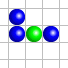
\includegraphics[width=0.5\textwidth]{Gol-born}
\caption{Une cellule nait}
\label{alive}
\end{minipage}
\hspace{0.5cm}
\begin{minipage}{0.3\textwidth}
\centering
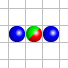
\includegraphics[width=0.5\textwidth]{Gol-nochange}
\caption{Conservation d'un état}
\label{nochange}
\end{minipage}
\hspace{0.5cm}
\begin{minipage}{.3\textwidth}
\centering
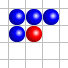
\includegraphics[width=0.5\textwidth]{Gol-dead}
\caption{Une cellule meurt}
\label{dead}
\end{minipage}
\end{figure}

A partir de cet énoncé, une version séquentielle du jeu de la vie a été fabriquée. Nous nous sommes basés sur cette version pour paralléliser les calculs.


\section{Implémentation des différentes versions} % (fold)
\label{sec:diff_rents_versions}
Dans cette partie, nous allons exposer les différentes versions parallèles du jeu de la vie que nous avons développées. Dans un premier temps, nous allons voir les différentes versions utilisant une mémoire partagée (section \ref{partagee}), puis les version \texttt{MPI} (section \ref{mpi}), utilisant d'abord des communications synchrones, puis des communications asynchrones, et enfin persistantes. Le code itère sur une boucle incrémentant une variable $loop$ qui indique combien de fois on a effectué l'actualisation du plateau. Nous nous intéressons surtout au code contenu dans cette boucle.

\subsection{Mémoire partagée}
\label{partagee}

\subsubsection{OpenMP}
\label{openmp}
\paragraph{Principe}
Dans le cas d'\texttt{OpenMP}, on va essayer de paralléliser les boucles de calcul du nombre de voisins et d'actualisation des cellules en fonction du nombre de voisins (figures \ref{boucle_voisins} et \ref{boucle_actualisation}), en distribuant les boucles sur un nombre prédéfini de threads. Pour cela, on spécifie simplement que l'on veut effectuer les boucles $for$ en parallèle avec l'instruction \ref{omp_parallel}, insérée juste avant les boucles. Dans le cas de l'exemple \ref{boucle_actualisation}, on veut calculer le nombre de cellules vivantes aussi. Pour ce faire, on effectue une réduction, employant l'opérateur addition sur la variable $num\_alive$. Le nombre de threads est fixé au tout début du programme, une fois les arguments passés en paramètre au programme lus. 

\begin{figure}[!ht]
\begin{lstlisting}
for (j = 1; j <= BS; j++) do
	for (i = 1; i <= BS; i++) do
		ngb( i, j ) =
			cell( i-1, j-1 ) + cell( i, j-1 ) + cell( i+1, j-1 ) +
			cell( i-1, j   ) +                  cell( i+1, j   ) +
			cell( i-1, j+1 ) + cell( i, j+1 ) + cell( i+1, j+1 );
	end do
end do
\end{lstlisting}
\caption{Boucle calculant le nombre de voisins}
\label{boucle_voisins}
\end{figure}


\begin{figure}[h!]
\begin{lstlisting}
for (j = 1; j <= BS; j++) do
	for (i = 1; i <= BS; i++) do
		if ( (ngb( i, j ) < 2) || (ngb( i, j ) > 3) ) then
			cell(i, j) = 0;
		else 
		if ((ngb( i, j )) == 3) then
			cell(i, j) = 1;
		fi
		if (cell(i, j) == 1) then
			num_alive ++;
		fi
	end do
end do
\end{lstlisting}
\caption{Boucle calculant l'état suivant des cellules et comptant le nombre de cellules vivantes}
\label{boucle_actualisation}
\end{figure}

\begin{figure}[h!]
\begin{lstlisting}
#pragma omp parallel for private(i,j)
\end{lstlisting}
\caption{Instruction \texttt{OpenMP}}
\label{omp_parallel}
\end{figure}

\paragraph{Pavage}
\label{pavage}
Nous avons implémenté une version \texttt{OpenMP} utilisant la notion de \emph{pavage}. Il s'agit de découper les boucles en $N$ plus petites boucles de taille définie $bs$ ($N = BS/bs$). Le but est de faire correspondre la taille des petites boucles avec la taille du cache, afin de bénéficier de ses performances. 

\subsubsection{\texttt{pthread}}
\label{pthread}

La version utilisant \texttt{pthread} découpe le plateau de jeu en plusieurs blocs. On associe un bloc à chaque thread du programme. Chaque thread calcule alors l'étape suivante pour son bloc. Ce découpage pose un problème de synchronisation entre les threads. En effet, si un thread modifie ses cellules alors qu'un autres n'a pas terminé de calculer son nombre de voisins, il est possible qu'il y ait des conflits sur les bords des blocs. La méthode retenue pour empêcher ces conflits est d'utiliser des barrières avec la bibliothèque \texttt{pthread}.

\subsection{Mémoire distribuée: \texttt{MPI}} % (fold)
\label{mpi}

Le but de cette version est de répartir les blocs de calcul sur plusieurs processeurs. Les processus ne contiennent dans cette version qu'un seul thread. On considère que les blocs sont tous de taille $m \times n$, $m$ le nombre de lignes et $n$ le nombre de colonnes. Des cases fantômes sont rajoutées tout autour du bloc, ce qui en fait des blocs de taille $(m+2) \times (n+2)$.

\paragraph{Communications synchrones}
Dans cette version, les communications sont synchrones. Pour cela, nous avons utilisé la fonction \emph{MPI\_Sendrecv}. \texttt{MPI} gère alors tout seul l'envoi et la réception sans créer de deadlocks. Nous aurions aussi pu, pour éviter les deadlocks, utiliser un système d'envoi des processus impairs puis pairs, ou encore faire en sorte qu'un processus reçoit avant d'envoyer (première version à préférer). 

\begin{figure}[!ht]
\begin{lstlisting}
Send(up,line[1])
Recv(up,line[0])
Send(down,line[m])
Recv(down,line[m+1])

for (j = 2; j < n; j++) do
	for (i = 2; i < m/2; i++) do
		calcul_nb_voisins(i,j);
	end do
end do

Waitall(1-4);

Send(left,column[1])
Recv(left,column[0])
Send(right,column[n-1])
Recv(right,column[n])

for (j = 2; j < n ; j++) do
	for (i = m/2; i <= m; i++) do
		calcul_nb_voisins(i,j);
	end do
	calcul_nb_voisins(1,j);
end do

Waitall(5-8);

for (j = 1; j <= n ; j+=n-1) do
	for (i = 1; i <= m; i++) do
		calcul_nb_voisins(i,j);
	end do
end do
\end{lstlisting}
\caption{Recouvrement des communications par des calculs}
\label{recouvrement}
\end{figure}


\paragraph{Communications asynchrones}
Pour bénéficier des communications asynchrones, il fallait recouvrir les communications par des calculs. Pour cela, nous effectuons d'abord la communication entre le processus situé au-dessus et celui en-dessous, pour ensuite communiquer avec les voisins de droite et de gauche. Nous pouvons alors recouvrir les communications avec le calcul des voisins (voir le code de la figure \ref{recouvrement}). 
Nous calculons la moîtié d'un bloc, sans les côtés, pendant la première partie des communications, puis le reste du bloc pendant la deuxième partie des communications, toujours sans les côtés de droite et de gauche (mais en faisant cette fois la ligne du haut et du bas, sans les extrêmes), pour enfin faire la colonne de droite et de gauche une fois que toutes les communications sont terminées. 
Dans le code de la figure \ref{recouvrement}, les $Send$ et $Recv$ sont tous asynchrones ($MPI\_Isend$ et $MPI\_Irecv$). On impose cependant une barrière permettant de s'assurer que ces communications sont finies (l. 12 et 27), lorsqu'on en a besoin pour la suite.

L'ordre des communications peut être résumé par le schéma de la figure \ref{fig:comm}. A noter que l'on envoie d'abord seulement les cellules que l'on connaît, ce qui constitue donc un envoie de taille $n$. Au deuxième tour de communications, l'envoi est de taille $m+2$.

\begin{figure}[!ht]
\centering
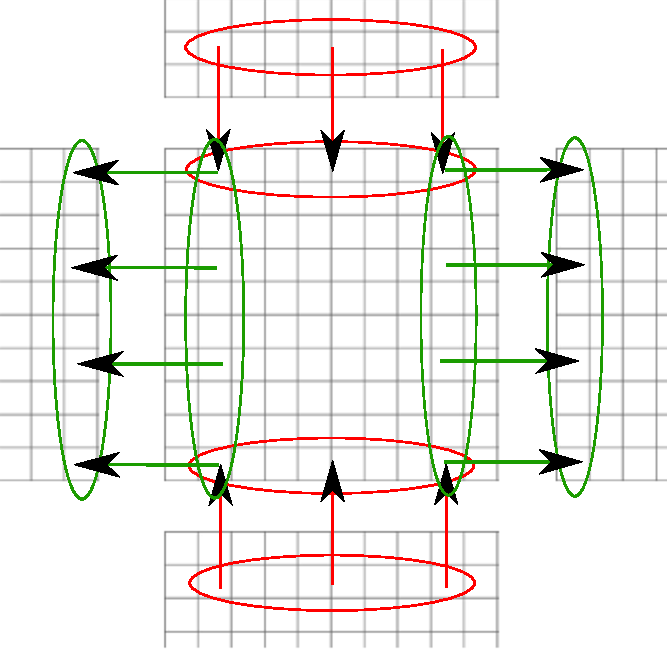
\includegraphics[width=0.6\textwidth]{comm.pdf}
\caption{Ordre des communications. Les rouges doivent se faire avant les vertes.}
\label{fig:comm}
\end{figure}

\paragraph{Communications persistantes}
Les communications sur la figure \ref{recouvrement}, des l. 1 à 4 et l. 14 à 17, sont remplacées par un simple $MPI\_Startall$, qui va lancer les requêtes, préparées à l'avance. De cette façon, les requêtes sont préparées dès le début du programme, une et une seule fois, et non pas à chaque tour de boucle de la variable $loop$. 
\section{Performances} % (fold)
\label{sec:perf}

Les tests de performances ont été effectués sur la machine PlaFRIM, en utilisant 4 noeuds et 4 processeurs par noeuds.

La première version du code améliorée avec \texttt{OpenMP} donne des résultats intéressants, mais possibles à améliorer. Quand les blocs deviennent très grands les accès mémoire ralentissent le programme. L'idée est de séparer les calculs en blocs (pavage) pour réduire ces temps d'accès à la mémoire (seconde version \texttt{OpenMP}). Les tailles des blocs doivent être calées exactement sur la taille du cache. Une mauvaise taille entraîne une perte de performance, comme on peut le voir sur la figure \ref{fig:sp-thread}, où la taille des blocs était de $64$. Une autre possibilité disponible avec \texttt{OpenMP} est l'utilisation des tâches. On génère des tâches ayant des tailles de blocs optimales et on exécute ces tâches. Un des avantages d'\texttt{OpenMP} est de pouvoir définir facilement un nombre de threads quelconque.\\

Pour les performances obtenues avec \texttt{pthread}, elle sont similaires à \texttt{OpenMP} pour le même nombre de threads. En effet, les deux versions utilisent le même type de ressources pour améliorer le temps de calcul. Le programme \texttt{pthread} actuel utilise des barrières pour s'assurer que les calculs précédents ont été effectués (à la façon d'\texttt{OpenMP}). Il est possible, avec un sémaphore par thread, de limiter les attentes à la terminaison des blocs adjacents et ainsi pour voir commencer l'étape suivante alors que certains threads n'ont pas terminé la précédente. Comme le nombre de threads disponibles sur un processeur ne peut pas dépasser une certaine valeur, il est plus intéressant (dans le cas des sémaphores) d'utiliser des blocs colonnes (car les matrices sont stockées en colonne dans notre projet). Enfin les blocs de threads ayant une taille dépendant de la matrice, il faudrait découper ces blocs en sous-blocs pour pouvoir optimiser les accès à la mémoire (même idée que le pavage, § \ref{pavage}). On peut remarquer que la version pthread est légèrement meilleure aux pics de performance, ceci est causé par la surcouche apportée par \texttt{OpenMP}, à l'inverse, quand le nombre de thread n'est pas optimal, \texttt{OpenMP} est légèrement devant.

\begin{figure}[!ht]
\centering
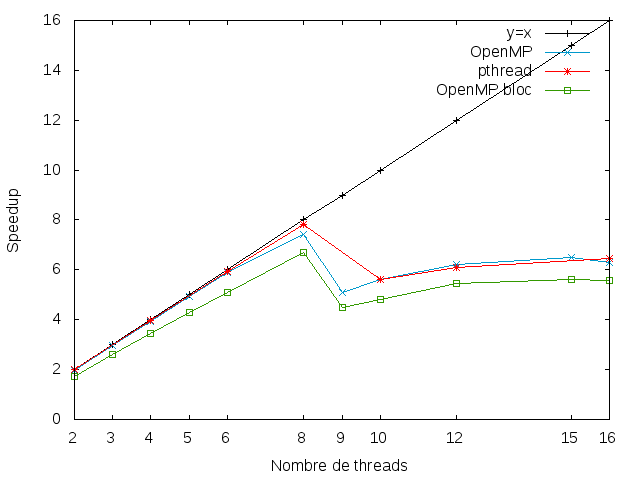
\includegraphics[width=0.8\textwidth]{speedup-thread.png}
\caption{Speed up des versions à mémoire partagée}
\label{fig:sp-thread}
\end{figure}

La figure \ref{fig:sp-thread} montre les résultats obtenus pour les versions à mémoire partagée (OpenMP et pthread) en faisant varier le nombre de threads. La largeur du plateau de jeu est alors 3600 cellules.
On remarque une chute lorsque l'on passe de 8 à 9 threads. Les machines ne pouvant faire tourner que 8 threads, la chute semble logique, car le problème sera moins bien découpé et un des threads devra attendre que les autres terminent avant de pouvoir s'exécuter.\\

Les performances de la version \texttt{MPI} sont meilleures que celles des versions multi-threadées. \texttt{MPI} permet à un nombre illimité de processus de s'exécuter en parallèle et donc de dépasser les accélérations des autres versions. Les trois versions de \texttt{MPI} ont des performances sensiblement identiques car les matrices testées ne sont pas exceptionnellement grandes et le nombre de processus reste relativement faible comparé à un gros calculateur. Cependant, la version synchrone avec les communications bloquantes reste la moins efficace, puisqu'elle ne fait rien durant ses communications. La différence entre la version asynchrone et la version persistante est la rapidité d'exécution des communications. La version persistante n'a pas besoin de copier les buffers et de préparer les requêtes ; le programme gagne donc un peu de temps, mais cela n'est visible que sur de longues exécutions avec beaucoup de communications.
La figure \ref{fig:sp-proc} montre les performances des différentes versions \texttt{MPI} pour un plateau de jeu d'une largeur de 3600 cellules aussi, en faisant varier le nombre de processus. On peut voir que les courbes suivent la tendance de $y=x$, et décrochent un peu vers la fin, probablement à cause d'un surcoût de communications (en effet la version synchrone est plus faible que les autres).

\begin{figure}[H]
\centering
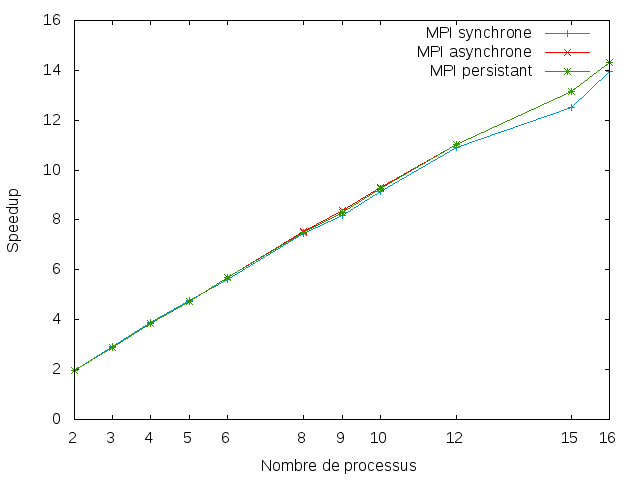
\includegraphics[width=0.8\textwidth]{speedup-mpi.png}
\caption{Speed up des versions multi-processus}
\label{fig:sp-proc}
\end{figure}

On peut aussi noter que le speedup est croissant avec la taille de plateau utilisée(Fig. \ref{sp-mpi-size}, \ref{sp-thread-size}). Dans ces tests, le nombre de processus/threads utilisé est 8. Le speedup s'approche (mais n'atteint pas) ce nombre de 8. S'il l'atteignait, cela signifierait une efficacité de 1, ce qui serait du parallélisme parfait.

\begin{figure}[H]
\centering
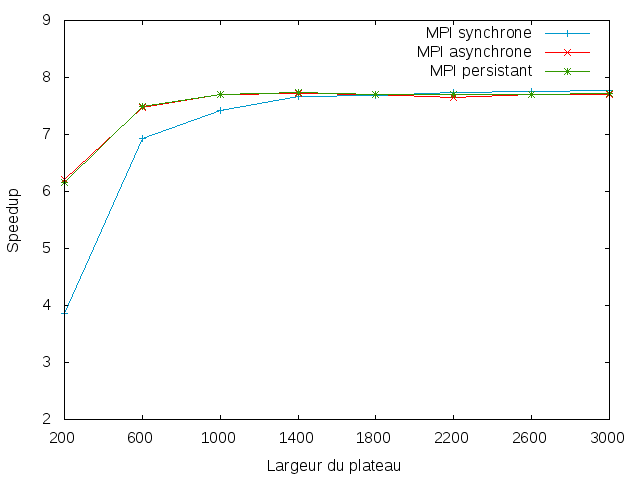
\includegraphics[width=0.8\textwidth]{sp-mpi-size.png}
\caption{Speed up de MPI avec une taille de plateau variable}
\label{sp-mpi-size}
\end{figure}
\begin{figure}[H]
\centering
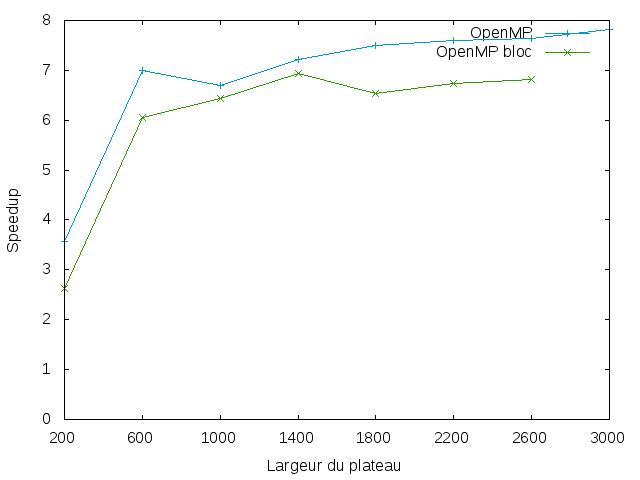
\includegraphics[width=0.8\textwidth]{sp-thread-size.png}
\caption{Speed up d'OpenMP avec une taille de plateau variable}
\label{sp-thread-size}
\end{figure}

La meilleure solution est de combiner \texttt{MPI}, avec des communications persistantes, avec \texttt{OpenMP} ou \texttt{pthread} pour multiplier les gains de performance, puisqu'un processus \texttt{MPI} s'exécute sur un c\oe ur qui peut avoir plusieurs threads.


\section{Discussion} % (fold)
\label{sec:discussion}

Le sujet évoquait le problème de charge inégale des calculs. En effet, dans certaines zones du plateau de jeu, il peut y avoir très peu de calcul. Lorsque, entre deux pas de la variable $loop$, il n'y a pas de changement pour une zone, on sait que celle-ci ne changera plus tant que ses bordures ne changent pas (donc lors d'échanges avec ses voisins). Cela permet d'effectuer un peu moins de calcul.

Cependant, dans notre implémentation actuelle, toutes les zones sont censées être calculées en parallèle. Et dans ce cas, qu'une zone ne travaille pas alors que ses voisins travaillent ne change rien en terme de temps d'exécution, bien que certains processus puissent se ``reposer'' un peu. 

Si les processus et leurs threads pouvaient se répartir mieux la charge de travail, on pourrait par contre gagner en performances. Plusieurs procédés existent pour cela, que nous avons pu voir au travers des différents TDPs. Le vol de travail permettrait aux processus inactifs de faire quelque chose au lieu d'être inactif, tout en réduisant la charge de travail d'un autre. 

Dans les versions \texttt{MPI} que nous avons écrites, les processus ne contenaient qu'une zone à calculer, comme cela était demandé par le sujet. Il serait probablement plus intéressant de donner plusieurs zones du plateau à chaque processus. Celui-ci se chargerait ensuite de les calculer, en les répartissant par exemple parmi ses threads. 

Il est probable qu'une zone où il ne se passe rien sur un long moment soit au milieu d'une plus grande zone inactive. Dans ce cas, si un processus contient toutes ces zones connexes inactives, il ne fera rien tandis que les autres processus travaillent.

Dans le cadre de cette idée, au lieu de répartir les processus sur une grille de façon ``linéaire'', nous pourrions utiliser une répartition en serpentin, ou en bloc-cyclique, afin de pallier le problème. Il est possible aussi d'utiliser une répartition pseudo-aléatoire, par exemple en usant du théorème de restes chinois. Les zones inactives seront alors bien réparties entre les processus. Un processus aura donc plus de chance d'avoir du travail. 




\end{document}
